\frametitle{Docking results of Phenytoin}
\begin{columns}
	\begin{column}{0.6\linewidth}
		\begin{figure}
			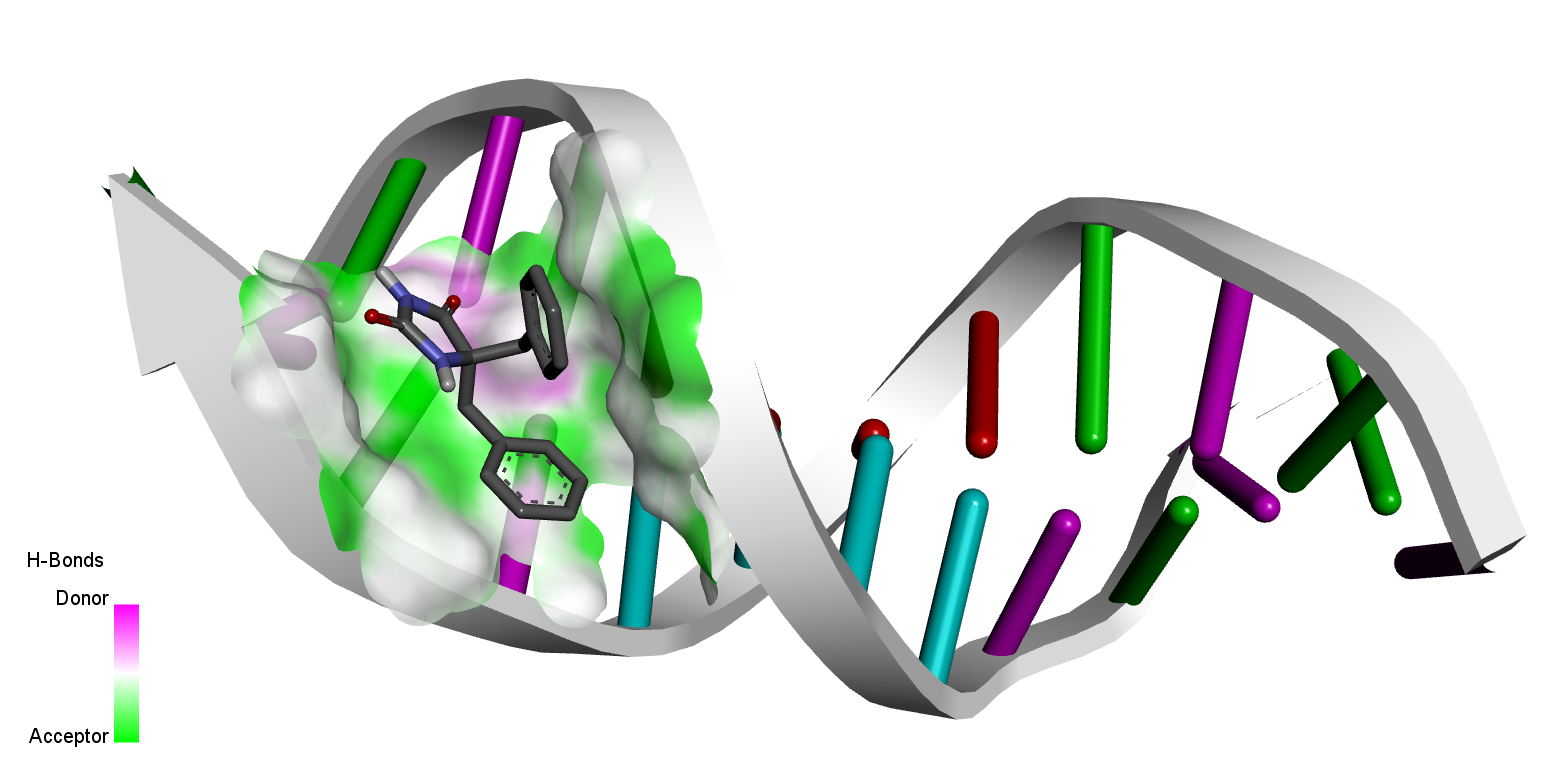
\includegraphics[width=\linewidth]{phenytoin-donor-acceptor.png}
			\caption{\centering The donor-acceptor interaction \linebreak between Phenytoin and B-DNA.}
			\label{fig:pht_donor_acceptor}
		\end{figure}
	\end{column}
	\begin{column}{0.45\linewidth}
		\centering
		\scriptsize
		\begin{table}
			\begin{tabular}{*{4}{c}}
				\hline\\[-1em]
				\multirow{2}{2em}{\centering\textbf{Mode}}&\multirow{2}{4em}{\centering\textbf{Affinity (kcal/mol)}}&\multicolumn{2}{c}{\centering\textbf{Distance from best mode}}\\
				\cline{3-4}
				&&\textbf{rmsd l.b.}&\textbf{rmsd u.b.}\\
				1&-5.8&0.000&0.000\\
				2&-5.7&2.433&3.604\\
				3&-5.7&2.081&5.276\\
				4&-5.7&2.863&4.281\\
				5&-5.5&2.633&3.968\\
				6&-5.5&2.360&3.522\\
				7&-5.4&1.717&2.503\\
				8&-5.4&2.296&4.480\\
				9&-5.3&2.010&3.798\\
				\hline
			\end{tabular}
			\caption{\centering The binding affinities and RMSD values between Phenytoin and B-DNA.}
			\label{table:pht}
		\end{table}
	\end{column}
\end{columns}